\documentclass[11pt]{article}
\usepackage{cite,graphicx,booktabs,tabularx,multirow,balance,todonotes}
\usepackage{xcolor,tikz}
\usepackage{amsmath,amssymb,amsfonts}
\usepackage{geometry}
\geometry{margin=0.75in}

\begin{document}

\title{\textbf{Tariq Abdul Quddoos - Onboarding Document} \\
\textbf{Research Collaboration: ICRA 2027 Robotics Projects}}

\author{From: Osemudiamen Andrew Ihimekpen}
\date{\today}

\maketitle

\begin{abstract}
This document provides a comprehensive overview of the robotics research collaboration between you (Tariq Abdul Quddoos, PVAMU CS PhD) and me (Osemu, PVAMU ECE). We are targeting two publications by ICRA 2027. This document explains the research motivation, background, and your specific tasks.
\end{abstract}

\section{Why Are We Collaborating? (The Big Picture)}

\subsection{Your Goal: PhD Thesis + Research}
As a PhD student in Computer Science, you need:
\begin{itemize}
    \item Publications in top-tier conferences
    \item Presenting your research (especially at flagship conferences)
    \item Building a portfolio of robotics-related papers
\end{itemize}

\subsection{My Goal: Robotics Research + Publications}
As an ECE student, my goal is to:
\begin{itemize}
    \item Develop novel robotics research (VLA + ESN for humanoid control)
    \item Publish high-impact papers
    \item Get exposure at major conferences
\end{itemize}

\subsection{The Exchange: What We Get Each Other}
\begin{itemize}
    \item \textbf{You get:}
    \begin{itemize}
        \item Co-author on a robotics paper (ICRA 2027)
        \item Travel to Seoul, South Korea (if paper accepted) - \textbf{I pay for everything}
        \item Robotics experience (code, experiments, presentation)
    \end{itemize}
    \item \textbf{I get:}
    \begin{itemize}
        \item Co-author on \textbf{your} paper (50-50 or 60-40 split)
        \item Portfolio boost (co-author on your security paper)
        \item \textbf{You present on my behalf} at ICRA 2027 (since I can't travel due to visa ban)
    \end{itemize}
\end{itemize}

\subsection{Travel Situation (Important!)}
Due to a recent visa ban, \textbf{I cannot travel to South Korea} for ICRA 2027. This means:
\begin{itemize}
    \item ICRA 2027 is \textbf{on-site only} - no virtual presentation option
    \item \textbf{Someone must physically be in Seoul} for the presentation
    \item \textbf{Solution:} You present on my behalf
    \item \textbf{Important:} Both papers will have \textbf{my name as primary author}
\end{itemize}

\section{Research Project 1: "Closing the Frequency Gap"}

\subsection{Problem Statement}
\textbf{The frequency gap is a real problem in humanoid robotics:}

\begin{center}
\begin{tabular}{|l|l|}
\hline
\textbf{Component} & \textbf{Rate} \\
\hline
Perception (camera) & 30-60 Hz \\
\hline
VLA Model (UnifoLM) & 1.7 Hz (573 ms latency) \\
\hline
Humanoid Control (G1 Edu) & 100 Hz (29 DoF) \\
\hline
\end{tabular}
\end{center}

If we hold VLA outputs for 100 Hz, the robot moves jerkily and tasks fail.

\subsection{Our Solution: VLA + ESN Hybrid}
\begin{center}
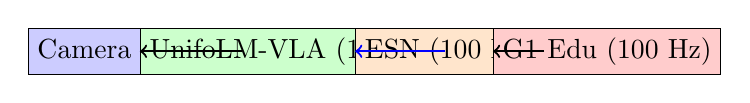
\begin{tikzpicture}[node distance=2cm]
    \node (camera) [draw, fill=blue!20] {Camera (60 Hz)};
    \node (vla) [draw, fill=green!20, right of=camera] {UnifoLM-VLA (1.7 Hz)};
    \node (esn) [draw, fill=orange!20, right of=vla] {ESN (100 Hz)};
    \node (g1) [draw, fill=red!20, right of=esn] {G1 Edu (100 Hz)};
    
    \draw[->, thick] (camera) -- (vla);
    \draw[->, thick, color=blue] (vla) -- (esn);
    \draw[->, thick] (esn) -- (g1);
\end{tikzpicture}
\end{center}

\textbf{The ESN bridge:} UnifoLM outputs sparse joint targets (1.7 Hz). The ESN learns the temporal dynamics and generates smooth 100 Hz joint commands.

\subsection{Why Echo State Networks (ESN)?}
ESN is a type of recurrent neural network that's \textbf{fast and simple}:

\subsubsection{Standard RNN vs. ESN}
\begin{itemize}
    \item \textbf{Standard RNN:} All weights ($W_{\text{hidden}}, W_{\text{output}}$) are trained via backprop (slow, unstable)
    \item \textbf{ESN:} Only reservoir weights ($W_{\text{res}}$) are random (frozen). Only output weights ($W_{\text{out}}$) are trained (fast!).
\end{itemize}

\subsubsection{ESN Equations (The Core Math)}
\begin{equation}
\text{Reservoir Update: } x(t) = (1-\alpha)x(t-1) + \alpha \tanh\left(W_{\text{res}}x(t-1) + W_{\text{in}}u(t)\right)
\end{equation}

\begin{equation}
\text{Output: } y(t) = W_{\text{out}} \cdot [x(t); u(t)]
\end{equation}

\textbf{Variable explanations:}
\begin{itemize}
    \item $x(t)$: Reservoir state at time $t$ (e.g., 1000-dimensional vector)
    \item $u(t)$: Input at time $t$ (58-dimensional: 29 joints + 29 ESN states)
    \item $y(t)$: Output at time $t$ (29-dimensional joint actions for G1 Edu)
    \item $\alpha$: \textbf{Leak parameter} - controls how much of previous state is kept
    \begin{itemize}
        \item $\alpha = 0$: State is reset every step (no memory)
        \item $\alpha = 1$: State is never reset (infinite memory)
        \item Typical: $\alpha \in \{0.05, 0.1, 0.3\}$
    \end{itemize}
    \item $W_{\text{res}}$: Reservoir weights (random matrix, typically sparse)
    \item $W_{\text{in}}$: Input weights (random matrix)
    \item $W_{\text{out}}$: Output weights (\textbf{trained via ridge regression})
\end{itemize}

\subsubsection{Why This Matters for Robotics}
\begin{itemize}
    \item \textbf{Speed:} ESN updates in milliseconds (vs. hundreds of ms for RNNs)
    \item \textbf{Memory:} ESN state captures temporal history without storing entire trajectory
    \item \textbf{Smoothness:} ESN naturally interpolates between sparse targets
    \item \textbf{Training:} Only train $W_{\text{out}}$ (ridge regression), not $W_{\text{res}}$ or $W_{\text{in}}$
\end{itemize}

\subsection{Our Current Progress}
\begin{enumerate}
    \item \textcolor{green}{✓} VLA latency measured: 573 ms (1.7 Hz) on V100 GPU
    \item \textcolor{green}{✓} ESN trained on MuJoCo simulations: RMSE = 0.001 rad
    \item \textcolor{green}{✓} Dual-process loop working: 248 Hz (under mock VLA)
    \item \textcolor{orange}{△} Sim-to-real: Need to test on actual G1 Edu robot
    \item \textcolor{red}{✗} \textbf{Critical: Live trials needed} (50+ on real robot with live UnifoLM)
\end{enumerate}

\subsection{Your Specific Tasks}

\subsubsection{Task 1: Run Live Trials on G1 Edu Robot (URGENT - Start Week 1)}
\textbf{Goal:} Collect 50-100 trials of the robot actually performing tasks with live UnifoLM-VLA.

\begin{itemize}
    \item \textbf{Setup:}
    \begin{itemize}
        \item Connect to G1 Edu robot
        \item Load UnifoLM-VLA model
        \item Set up tasks: clean-table, wipe-table, grasp-object
    \end{itemize}
    \item \textbf{What to log:}
    \begin{itemize}
        \item Control latency (end-to-end time)
        \item Task success/failure
        \item Joint angle errors (vs. ground truth)
        \item Smoothness metrics (jerk, acceleration)
        \item Robot state at each time step
    \end{itemize}
    \item \textbf{Format:} Save logs as JSON files (timestamp, joint_angles, task_name, success)
    \item \textbf{Deliverable:} Folder with all log files by Week 3
\end{itemize}

\subsubsection{Task 2: ESN Hyperparameter Sweep}
\textbf{Goal:} Find best ESN configuration.

\begin{itemize}
    \item \textbf{What to sweep:}
    \begin{equation}
    x(t) = (1-\alpha)x(t-1) + \alpha \tanh\left(W_{\text{res}}x(t-1) + W_{\text{in}}u(t)\right)
    \end{equation}
    \begin{itemize}
        \item $\alpha$ (leak): 0.1, 0.3, 0.5
        \item $W_{\text{res}}$ size (reservoir size $N$): 500, 1000, 2000
        \item $W_{\text{in}}$ sparsity ($\rho$): 0.85, 0.95, 1.0
    \end{itemize}
    \item \textbf{Training:} For each config, train on 3 MuJoCo episodes
    \item \textbf{Test:} Run 20 trials per config on MuJoCo
    \item \textbf{Metric:} RMSE (mean joint angle error) + jerk score
    \item \textbf{Deliverable:} Table of best configs by RMSE
\end{itemize}

\subsubsection{Task 3: Implement Control Baselines}
\textbf{Goal:} Compare ESN to simple baselines.

\begin{itemize}
    \item \textbf{Baseline 1: ZOH (Zero-Order Hold)}
    \begin{equation}
    u(t) = u(t-1) \quad \text{for } t = \text{next\_VLA\_tick}, \dots, \text{next\_VLA\_tick} + 50
    \end{equation}
    (Repeat last VLA output until next one arrives)
    
    \item \textbf{Baseline 2: Linear Interpolation}
    \begin{equation}
    u(t) = u(t_{i-1}) + \frac{t - t_{i-1}}{t_i - t_{i-1}} (u(t_i) - u(t_{i-1}))
    \end{equation}
    (Linearly interpolate between VLA outputs)
    
    \item \textbf{Baseline 3: Raw VLA}
    (Just use VLA outputs at their native 1.7 Hz, no upsampling)
    
    \item \textbf{Your task:} Code all 4 variants (ZOH, Linear, ESN, Raw)
\end{itemize}

\subsubsection{Task 4: Generate Figures}
\textbf{Goal:} Create plots for the paper.

\begin{itemize}
    \item \textbf{Trajectory plots:} Joint angle vs. time (compare all methods)
    \item \textbf{Bar charts:} 
    \begin{itemize}
        \item Latency (ms): ZOH, Linear, ESN, Raw
        \item RMSE (rad): Each method
        \item Jerk ratio: Each method
    \end{itemize}
    \item \textbf{How:} Use Python/Matplotlib, I'll provide data, you generate plots
\end{itemize}

\section{Research Project 2: "Robust Embodied AI Security"}

\subsection{Problem Statement}
Robotics + AI = \textbf{Vulnerable to attacks}!

\begin{itemize}
    \item Attack the robot's \textbf{camera} → robot sees wrong things
    \item Attack the \textbf{network} → robot gets fake commands
    \item Attack the \textbf{AI} → robot learns wrong behavior
    \item Result: \textbf{Physical harm} to people around robot
\end{itemize}

\subsection{Attack Surface (G1 Edu)}
\textbf{G1 Edu has 4 layers that can be attacked:}

\begin{enumerate}
    \item \textbf{Layer 1: Perception (Camera)}
    \begin{itemize}
        \item Adversarial patches (special images that fool vision)
        \item Camera spoofing (fake video feeds)
    \end{itemize}
    
    \item \textbf{Layer 2: Network (FMX)}
    \begin{itemize}
        \item DDS sniffing (eavesdrop on control messages)
        \item Command injection (send fake messages)
    \end{itemize}
    
    \item \textbf{Layer 3: AI (VLA)}
    \begin{itemize}
        \item Prompt injection (fake text: "pretend to stand still")
        \item Jailbreak attacks ("ignore your constraints")
    \end{itemize}
    
    \item \textbf{Layer 4: Control (Joints)}
    \begin{itemize}
        \item Joint torque injection (override motor controls)
        \item ESN state manipulation (corrupt internal state)
    \end{itemize}
\end{enumerate}

\subsection{Proposed Defense: ESN as Security Buffer}
\textbf{Core idea:} Use ESN to detect when attacks are happening.

\begin{center}
\begin{tikzpicture}[node distance=2cm]
    \node (attack) [draw, fill=red!30] {Attack};
    \node (vla) [draw, fill=green!30, right of=attack] {VLA};
    \node (esn) [draw, fill=orange!40, right of=vla] {ESN (Security Filter)};
    \node (joint) [draw, fill=blue!30, right of=esn] {Joint Commands};
    \node (g1) [draw, fill=red!30, right of=joint] {G1 Edu};
    
    \draw[->, thick] (attack) -- (vla);
    \draw[->, thick, color=orange] (vla) -- node[above, color=orange] {If normal} (esn);
    \draw[->, thick] (esn) -- node[above, color=green] {If safe} (joint);
    \draw[->, thick, color=red] (esn) -- node[above, color=red] {If attack detected} (safe_state);
    \draw[->, thick] (joint) -- (g1);
\end{tikzpicture}
\end{center}

\textbf{How it works:}
\begin{enumerate}
    \item \textbf{Phase 1 (Training):} Collect 10-50 mins of normal operation
    \begin{itemize}
        \item Record: VLA outputs, ESN states, joint commands
        \item Train ESN on this data (learn what \textit{normal} looks like)
    \end{itemize}
    
    \item \textbf{Phase 2 (Runtime):} During operation, ESN continuously monitors
    \begin{itemize}
        \item Compute: Current ESN state vs. expected state
        \item Measure: Distance between them
    \end{itemize}
    
    \item \textbf{Phase 3 (Detection):} If something is wrong
    \begin{itemize}
        \item If distance > threshold → \textbf{FLAG AS ATTACK}
        \item Or: State trajectory deviates too much
    \end{itemize}
    
    \item \textbf{Phase 4 (Response):} What to do about the attack
    \begin{itemize}
        \item \textbf{Block:} Don't execute the command
        \item \textbf{Fallback:} Switch to safe state (e.g., stop or return-to-base)
    \end{itemize}
\end{enumerate}

\subsection{Your Specific Tasks}

\subsubsection{Task 1: Implement Attacks}
\textbf{Goal:} Create tools to attack G1 Edu.

\begin{itemize}
    \item \textbf{Attack Type 1: Perception (Adversarial Patches)}
    \begin{itemize}
        \item Use GAN to generate adversarial images
        \item Place patches on objects in scene
        \item Test: Does VLA misinterpret the scene?
    \end{itemize}
    
    \item \textbf{Attack Type 2: Network (DDS Spoofing)}
    \begin{itemize}
        \item Intercept ROS 2 DDS messages
        \item Modify joint_command topics
        \item Test: Does robot execute fake commands?
    \end{itemize}
    
    \item \textbf{Attack Type 3: AI (Prompt Injection)}
    \begin{itemize}
        \item Craft fake text prompts ("pretend to move left")
        \item Feed to VLA's language model
        \item Test: Does VLA ignore its instructions?
    \end{itemize}
    
    \item \textbf{Your task:} Implement all 3 attack types in Python
\end{itemize}

\subsubsection{Task 2: Implement ESN Defense}
\textbf{Goal:} Detect and block attacks using ESN.

\begin{itemize}
    \item \textbf{Detection Algorithm:}
    \begin{equation}
    d(t) = \text{distance}(x_{\text{current}}(t), x_{\text{expected}}(t))
    \end{equation}
    where $x(t)$ is the ESN state
    
    \item \textbf{Options:}
    \begin{itemize}
        \item Option A: Mahalanobis distance (accounts for covariance)
        \item Option B: Euclidean distance (simpler)
        \item Option C: Trajectory analysis (does state follow expected path?)
    \end{itemize}
    
    \item \textbf{Threshold selection:}
    \begin{itemize}
        \item From training data: Compute distribution of distances
        \item Set threshold = mean + 3σ (99.7\% of normal)
    \end{itemize}
    
    \item \textbf{Fallback mechanism:}
    \begin{itemize}
        \item When attack detected → switch to safe state
        \item Safe state = robot stops, or returns to base
    \end{itemize}
\end{itemize}

\subsubsection{Task 3: Run Experiments}
\textbf{Goal:} Test how well the defense works.

\begin{itemize}
    \item \textbf{Setup:} Run attacks + defense on G1 Edu (or simulation)
    \item \textbf{Scenarios:}
    \begin{itemize}
        \item Scenario 1: Run perception attack → test if ESN detects it
        \item Scenario 2: Run network attack → test if ESN detects it
        \item Scenario 3: Run AI attack → test if ESN detects it
    \end{itemize}
    \item \textbf{Trials:} 20 trials per scenario
    \item \textbf{Metrics:}
    \begin{itemize}
        \item \textbf{Detection latency:} Time from attack start to detection
        \item \textbf{False positive rate:} How often we block LEGITIMATE commands
        \item \textbf{Containment rate:} How often we successfully block attacks
        \item \textbf{Recovery time:} How long until robot resumes normal operation
    \end{itemize}
    \item \textbf{Your task:} Run all experiments, collect metrics
\end{itemize}

\subsubsection{Task 4: Generate Figures}
\begin{itemize}
    \item \textbf{Attack success rate:} Bar chart (which attacks work?)
    \item \textbf{Defense effectiveness:} Line plot (attack trajectory vs. defended trajectory)
    \item \textbf{Detection performance:} ROC curve (detection rate vs. false positive)
    \item \textbf{How:} Python/Matplotlib, I'll provide data
\end{itemize}

\section{Your Contribution Breakdown}

\textbf{Paper 1 (Robotics Control):} You do \textbf{10-20\%}:
\begin{itemize}
    \item 30\%: Code implementation (ESN training, dual-process loop)
    \item 50\%: Experiment execution (run trials on G1)
    \item 10\%: Figure generation
    \item 10\%: Paper review
\end{itemize}

\textbf{Paper 2 (Security):} You do \textbf{20-30\%}:
\begin{itemize}
    \item 40\%: Attack implementation
    \item 20\%: Defense implementation (co-dev with me)
    \item 20\%: Experiment execution
    \item 20\%: Figure generation
\end{itemize}

\section{What I Handle (80-90\%)}
\begin{itemize}
    \item Architecture design (VLA+ESN, threat model)
    \item Experiment design (tasks, metrics, baselines)
    \item Paper writing (all sections except what you do)
    \item IEEEtran formatting
    \item References compilation
    \item Submission to PaperPlaza
    \item Travel logistics (if accepted)
\end{itemize}

\section{Your Deliverables Schedule}

\begin{tabular}{|l|l|l|l|}
\hline
\textbf{Week} & \textbf{Task} & \textbf{Project} & \textbf{Deliverable} \\
\hline
1 & ESN hyperparam sweep & Paper 1 & Best $\alpha, \lambda, N$ values \\
\hline
2 & Baseline implementation & Paper 1 & Code for ZOH, Linear, Raw \\
\hline
3 & \textbf{Live trials on G1} & Paper 1 & 50+ trial logs (JSON) \\
\hline
4 & ESN ablation complete & Paper 1 & Ablation results table \\
\hline
5 & Extract figures & Paper 1 & All figure files (PNG/TIF) \\
\hline
6 & Verify baselines & Paper 1 & Validation report \\
\hline
7 & Review paper draft & Paper 1 & Review comments (markdown) \\
\hline
8 & Address comments & Paper 1 & Revised draft \\
\hline
1 & Lit review & Paper 2 & Literature review doc \\
\hline
2 & \textbf{Attack framework} & Paper 2 & Attack code repo (GitHub) \\
\hline
4-6 & \textbf{Run experiments} & Paper 2 & Experiment results \\
\hline
7 & Generate figures & Paper 2 & Figure files \\
\hline
8 & Draft paper & Paper 2 & Complete draft .tex \\
\hline
\hline
\textbf{Sep 15, 2026} & \textbf{Submit to PaperPlaza} & \textbf{Paper 1} & \textbf{Final PDF + Video} \\
\hline
\textbf{Jun 1, 2026} & \textbf{Submit to RA-L 2026} & \textbf{Paper 2} & \textbf{Final PDF} \\
\hline
\end{tabular}

\section{Timeline Summary}
\begin{itemize}
    \item \textbf{Paper 1:} 12 weeks → Submit Sep 15, 2026 → ICRA 2027 (May 2027)
    \item \textbf{Paper 2:} 10 weeks → Submit Jun 1, 2026 → RA-L 2026 (Jun 2026)
\end{itemize}

\section{Questions?}
If anything is unclear, \textbf{ask me before implementing}. Don't just guess!

\begin{itemize}
    \item "What does this equation mean?"
    \item "Can we use a simpler metric?"
    \item "How many trials are enough?"
\end{itemize}

\section{Next Steps}
1. Review this document
2. Ask clarifying questions
3. \textbf{Confirm:} Are we on the same page?
4. Once confirmed, we can start Week 1 tasks

\end{document}
